\chapter{Implementation}
\section{RAG Chatbot}
    \subsection{Chatbot Interface}
        The chatbot interface was developed using the \texttt{Streamlit} library, which provides a simple and interactive way to create web applications. The interface allows users to interact with the RAG chatbot by entering a question in the input field and receiving the corresponding answer from the model. The chatbot interface was designed to be user-friendly and intuitive, enabling users to easily communicate with the chatbot and obtain relevant information.
        \begin{figure}[H]
            \centering
            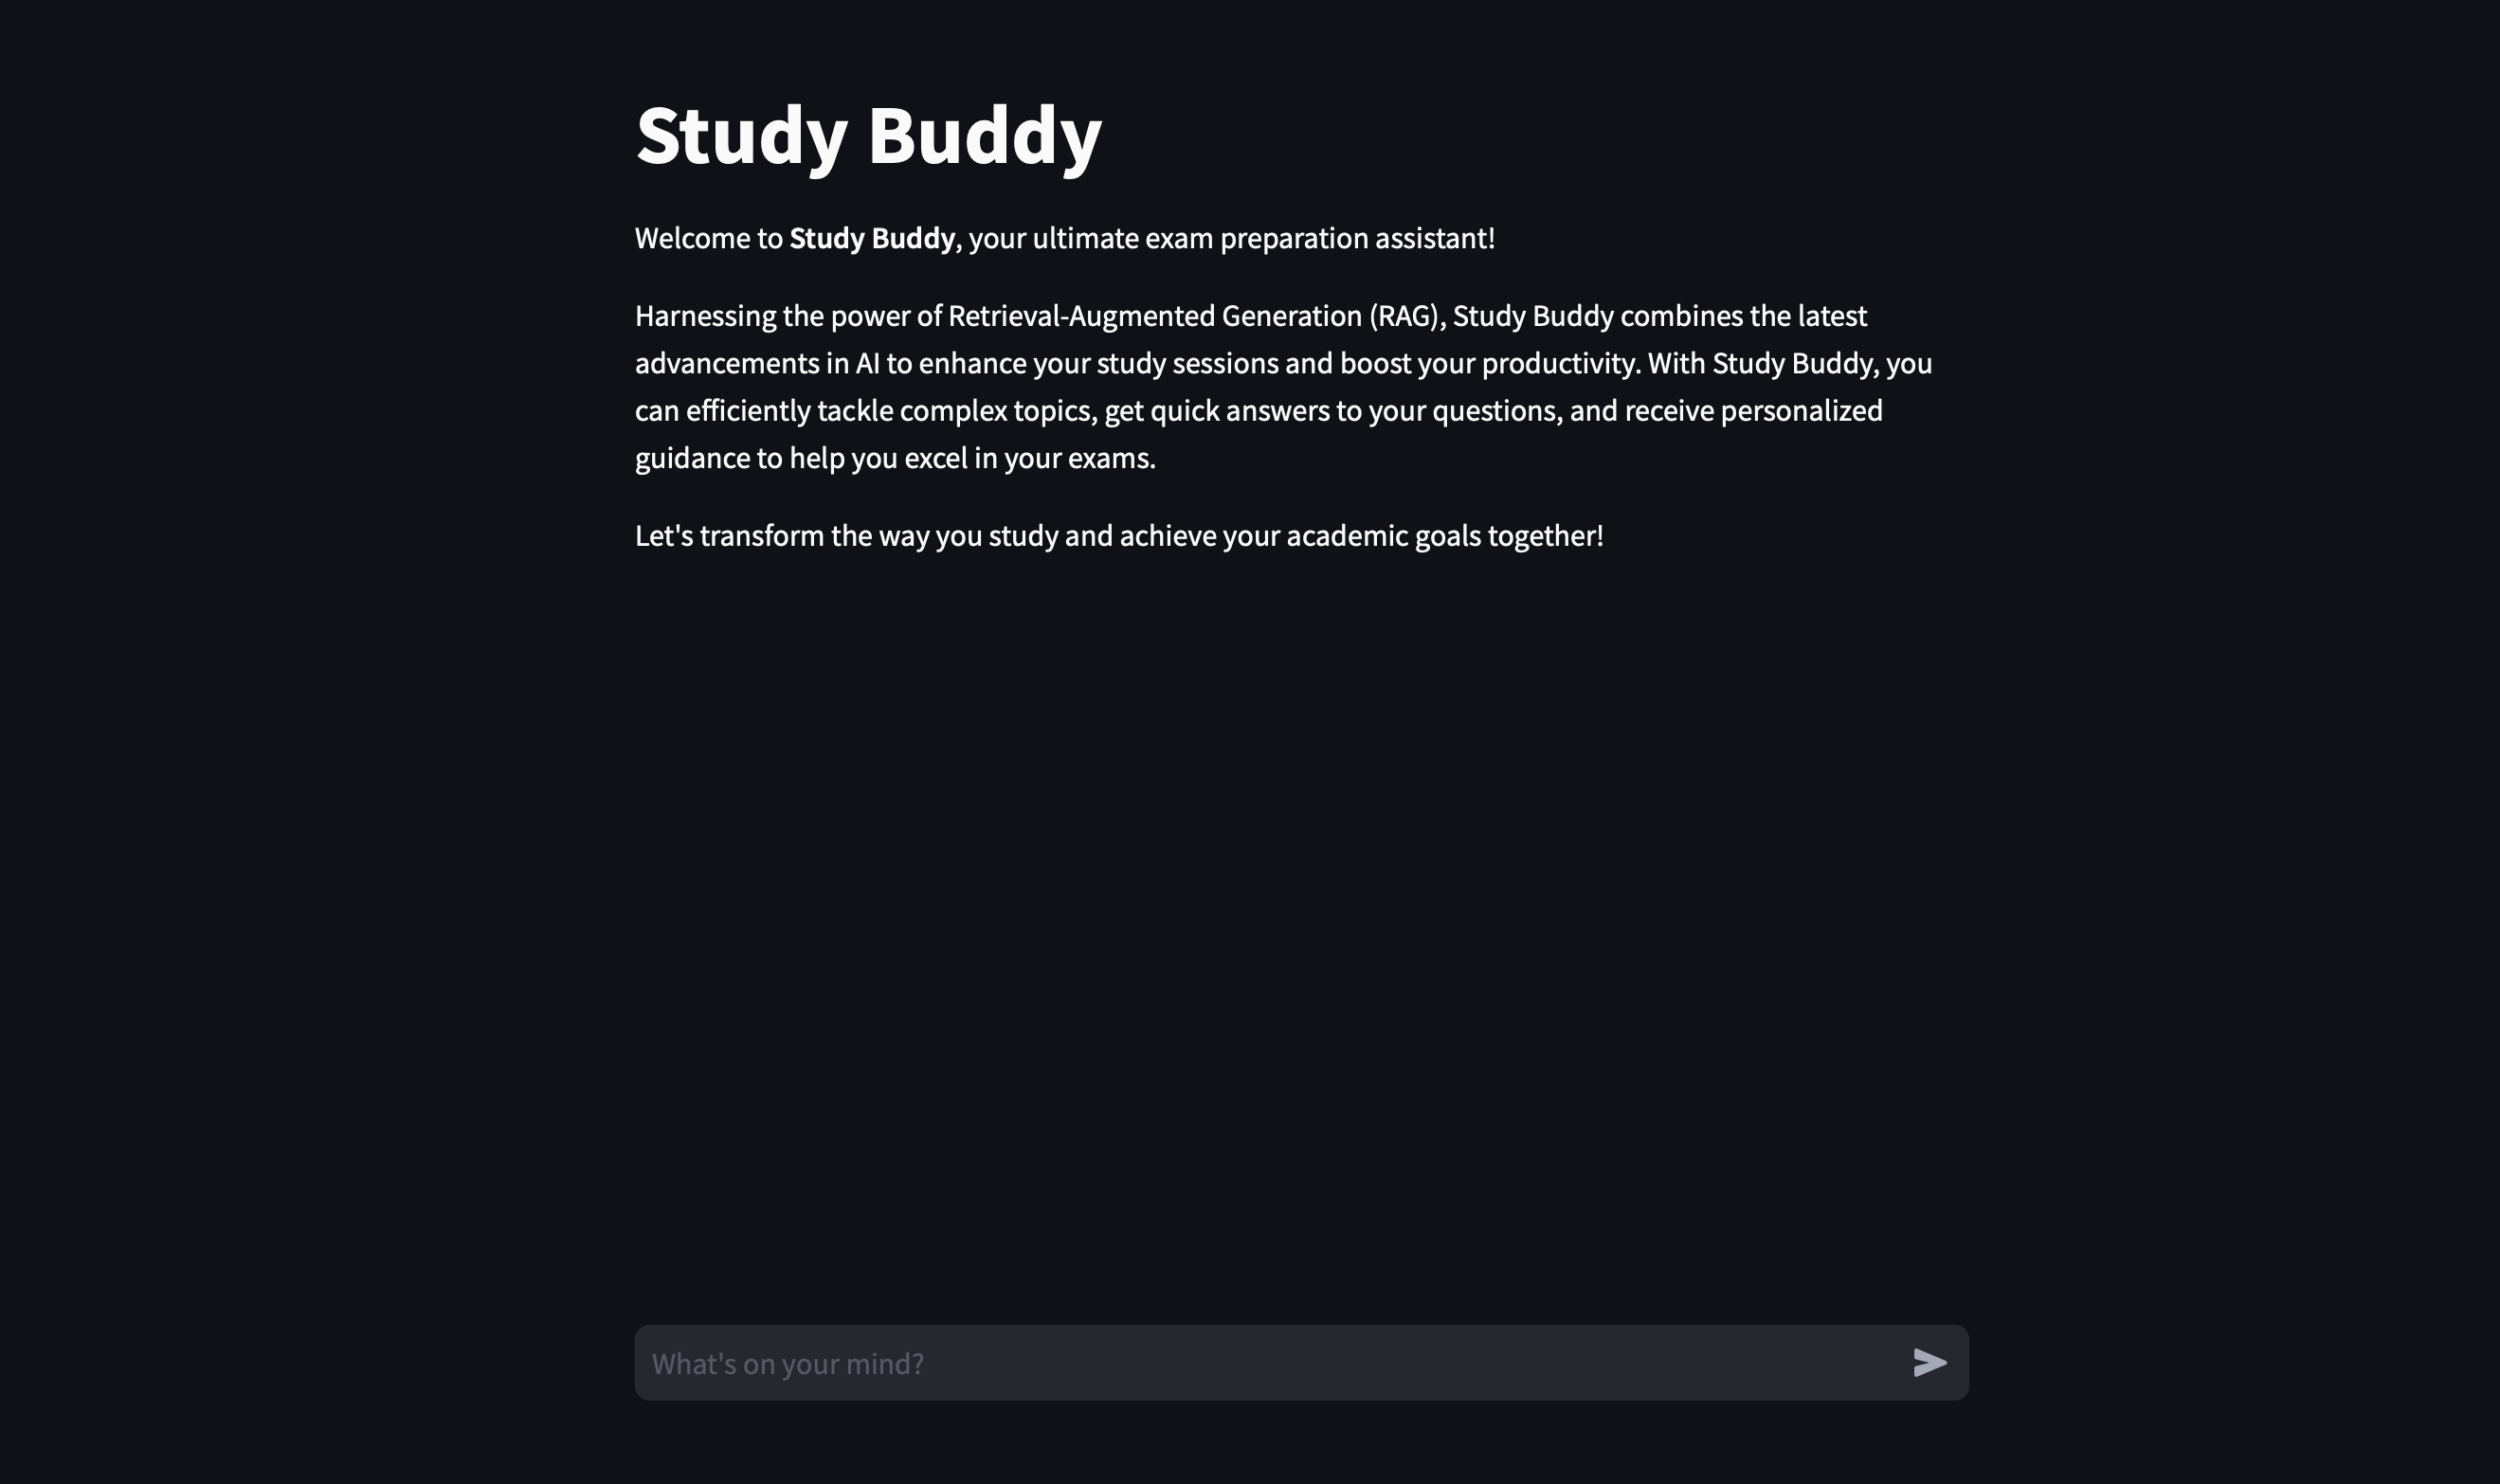
\includegraphics[width=0.8\textwidth]{figs/interface.png}
            \caption{RAG Chatbot Interface}
            \label{fig:chatbot_interface}
        \end{figure}
            
            The chatbot interface displays a title, description and input field for user queries using the \texttt{st.title}, \texttt{st.markdown} and \texttt{st.chat\_input} functions respectively. The title introduces the chatbot as "Study Buddy," while the description provides an overview of the chatbot's capabilities and features. By using the \texttt{Streamlit} library, the chatbot interface can be created by just a few lines of code.

\subsection{Generator Component}
The generator component of Study Buddy was implemented using the \texttt{Langchain} library, which provides ready-to-use methods to call OpenAI's GPT-4 model. Streamlit reruns the code in the \texttt{app.py} file every time a user interacts with the chatbot. The following code snippets demonstrate how the generator calls the GPT-4 model and generates responses to user queries.

\begin{listing}[H]
\begin{minted}[fontsize=\footnotesize]{python}
from langchain_openai import ChatOpenAI

# Cache OpenAI Chat Model for reuse
@st.cache_resource()
def get_chat_model():
    return ChatOpenAI(
        temperature=0.3,
        model='gpt-4',
        streaming=True,
        verbose=True
    )
chat_model_instance = get_chat_model()
\end{minted}
\caption{Caching the OpenAI Chat Model}
\label{listing:Cache_Chat_Model}
\end{listing}

The above code snippet details the implementation of the generator component for the Study Buddy chatbot, leveraging the \texttt{Langchain} library to interface with OpenAI's GPT-4 model. The generator component is responsible for producing the responses to user queries.

\textbf{Key Elements of the Code:}
\begin{itemize}
    \item \texttt{ChatOpenAI}: This class from the \texttt{langchain\_openai} module facilitates interaction with OpenAI's GPT-4 model.
    \item \texttt{@st.cache\_resource}: This Streamlit decorator caches the chat model instance, ensuring efficient reuse across multiple interactions without the need to reinitialize it each time.
    \item \texttt{temperature}: A parameter that controls the randomness of the model's responses, with a value of 0.3 indicating a balance between creativity and determinism.
    \item \texttt{model='gpt-4'}: Specifies the use of the GPT-4 model for generating responses.
    \item \texttt{streaming=True}: Enables streaming of the model's output, allowing for real-time response generation.
    \item \texttt{verbose=True}: Provides detailed logs of the model's operations for debugging and transparency.
\end{itemize}

\textbf{Explanation of Functionality:}
\begin{enumerate}
    \item \textbf{Caching the Chat Model:} The \texttt{get\_chat\_model()} function initializes and caches an instance of the GPT-4 model with specific parameters. By caching this instance, the system ensures that the model does not need to be reloaded each time a user interacts with the chatbot, thereby improving efficiency and response times.
    \item \textbf{Model Parameters:} The temperature parameter is set to 0.3, which strikes a balance between generating creative responses and maintaining consistency. The \texttt{streaming=True} parameter enables the model to stream responses in real-time, providing a more interactive and immediate user experience. The \texttt{verbose=True} parameter allows for detailed logging, which is useful for monitoring the chatbot's operations and debugging issues.
\end{enumerate}

This setup ensures that the generator component efficiently produces detailed and contextually relevant responses, enhancing the chatbot's effectiveness as an exam preparation assistant.

        
\subsection{Retriever Component}
The retriever component of Study Buddy was implemented using the \texttt{Langchain} library to retrieve the \(k = 5\) most relevant documents from the Astra DB Vector Store.

\begin{listing}[H]
\begin{minted}[fontsize=\footnotesize]{python}
from langchain_community.vectorstores import AstraDB
from langchain_openai import OpenAIEmbeddings

# Cache the Astra DB Vector Store for reuse
@st.cache_resource(show_spinner='Connecting to AstraDB')
def get_vector_store():
    vector_store_instance = AstraDB(
        embedding=OpenAIEmbeddings(),
        collection_name="datastax",
        api_endpoint=st.secrets['ASTRA_API_ENDPOINT'],
        token=st.secrets['ASTRA_TOKEN']
    )
    return vector_store_instance
vector_store_instance = get_vector_store()

# Cache the Retriever for reuse
@st.cache_resource(show_spinner='Initializing retriever')
def get_retriever():
    retriever_instance = vector_store_instance.as_retriever(
        search_kwargs={"k": 5}
    )
    return retriever_instance
retriever_instance = get_retriever()
\end{minted}
\caption{Caching the Astra DB Vector Store and Retriever}
\label{listing:Cache_Retriever}
\end{listing}

The above code snippet demonstrates the implementation of the retriever component for the Study Buddy chatbot. The \texttt{Langchain} library is utilized to connect to the Astra DB Vector Store, which is a database optimized for vector searches. The retriever component is responsible for identifying and retrieving the most relevant documents based on the user's query.

\textbf{Key Elements of the Code:}
\begin{itemize}
    \item \texttt{AstraDB}: This class from the \texttt{langchain\_community.vectorstores} module is used to create an instance of the vector store. It requires an embedding model, collection name, API endpoint, and token for authentication.
    \item \texttt{OpenAIEmbeddings}: This class from the \texttt{langchain\_openai} module provides the embedding model used to convert text into numerical vectors that the vector store can handle.
    \item \texttt{@st.cache\_resource}: This Streamlit decorator caches the resources, ensuring that the vector store and retriever instances are reused efficiently across different runs of the application. This caching mechanism helps to optimize performance by avoiding redundant connections and initializations.
    \item \texttt{get\_vector\_store()}: This function initializes and returns an instance of the vector store by connecting to Astra DB using the provided API endpoint and token.
    \item \texttt{get\_retriever()}: This function initializes and returns an instance of the retriever, configured to fetch the top \(k = 5\) most relevant documents based on the user's query.
\end{itemize}

\textbf{Explanation of Functionality:}
\begin{enumerate}
    \item \textbf{Connecting to Astra DB:} The \texttt{get\_vector\_store()} function creates a connection to the Astra DB Vector Store using the OpenAI embeddings for document vectorization. The connection details, such as the API endpoint and token, are securely retrieved from the Streamlit secrets configuration.
    \item \textbf{Initializing the Retriever:} The \texttt{get\_retriever()} function sets up the retriever to query the vector store. The retriever is configured to return the top 5 relevant documents, which helps in providing contextually accurate responses to user queries.
\end{enumerate}

This setup ensures that the retriever component can efficiently access and retrieve relevant information, enhancing the chatbot's ability to deliver detailed and context-specific answers.

\subsection{Integration of Generator and Retriever}
The generator and retriever components were integrated to provide a comprehensive response to user queries. The following code snippet demonstrates how the generator and retriever components work together to generate responses based on the user's input.

\begin{listing}[H]
\begin{minted}[fontsize=\footnotesize]{python}
from langchain.schema.runnable import RunnableMap

input_data = RunnableMap({
        'context': lambda x: retriever_instance.get_relevant_documents(x['question']),
        'question': lambda x: x['question']
    })
response_chain = input_data | chat_prompt | chat_model_instance
\end{minted}
\caption{Integration of Generator and Retriever}
\label{listing:Integration_Generator_Retriever}
\end{listing}

The above code snippet illustrates the integration of the generator and retriever components for the Study Buddy chatbot. This integration ensures that user queries are processed using both components to provide contextually accurate and comprehensive responses.

\textbf{Key Elements of the Code:}
\begin{itemize}
    \item \texttt{RunnableMap}: This class is used to map the inputs (context and question) to the necessary functions for processing.
    \item \texttt{retriever\_instance.get\_relevant\_documents}: This function retrieves the most relevant documents from the vector store based on the user's query.
    \item \texttt{chat\_prompt}: A predefined template that formats the retrieved context and user question for the generator.
    \item \texttt{chat\_model\_instance}: The cached instance of the GPT-4 model used for generating responses.
\end{itemize}

\textbf{Explanation of Functionality:}
\begin{enumerate}
    \item \textbf{Input Data Mapping:} The \texttt{RunnableMap} is used to create a mapping of inputs, where the 'context' key is assigned a lambda function that retrieves relevant documents based on the user's question, and the 'question' key simply maps the user's question.
    \item \textbf{Response Chain Creation:} The \texttt{response\_chain} is constructed by chaining the input data through the chat prompt and the chat model instance. This chain ensures that the user's question is enriched with relevant context before generating the final response.
    \item \textbf{Generating Responses:} When invoked, the \texttt{response\_chain} processes the inputs by first retrieving the relevant documents, then formatting them using the chat prompt, and finally generating a comprehensive response using the GPT-4 model.
\end{enumerate}

This integration of the generator and retriever components ensures that the Study Buddy chatbot can deliver detailed and contextually relevant answers to user queries, enhancing its utility as an exam preparation assistant.

\subsection{PDF Uploader}
The PDF uploader component allows users to upload course materials, lecture notes, or other relevant documents to the Study Buddy chatbot. The uploaded documents are stored in the Astra DB Vector Store, enabling the chatbot to retrieve and reference them when responding to user queries.

\begin{listing}[H]
\begin{minted}[fontsize=\footnotesize]{python}
# Sidebar for document upload
with st.sidebar:
    with st.form('upload_form'):
        uploaded_file = st.file_uploader('Upload a document for enhanced context', type=['pdf'])
        submit_button = st.form_submit_button('Save to AstraDB')
        if submit_button:
            process_and_vectorize_document(uploaded_file, vector_store_instance)
\end{minted}
\caption{PDF Uploader Interface}
\label{listing:PDF_Uploader}
\end{listing}
The above code snippet creates an interface within the Streamlit sidebar for uploading PDF documents. This interface allows users to upload course materials, lecture notes, or other relevant documents, which are then processed and stored in the Astra DB Vector Store.

\begin{listing}[H]
\begin{minted}[fontsize=\footnotesize]{python}
# Function to process and vectorize uploaded documents into Astra DB
def process_and_vectorize_document(uploaded_file, vector_db):
    if uploaded_file is not None:
        
        # Create a temporary file to store the uploaded document
        temp_dir = tempfile.TemporaryDirectory()
        temp_file_path = os.path.join(temp_dir.name, uploaded_file.name)
        with open(temp_file_path, 'wb') as temp_file:
            temp_file.write(uploaded_file.getvalue())

        # Load the PDF file
        document_pages = []
        pdf_loader = PyPDFLoader(temp_file_path)
        document_pages.extend(pdf_loader.load())

        # Initialize text splitter
        splitter = RecursiveCharacterTextSplitter(
            chunk_size=1500,
            chunk_overlap=100
        )

        # Split the document and add it to the vector store
        split_pages = splitter.split_documents(document_pages)
        vector_db.add_documents(split_pages)
        st.info(f"{len(split_pages)} pages have been loaded into the database.")
\end{minted}
\caption{Processing and Vectorizing Uploaded Documents}
\label{listing:Process_Vectorize_Documents}
\end{listing}

The above code snippet defines a function that processes and vectorizes uploaded PDF documents, storing them in the Astra DB Vector Store. This function is crucial for enabling the chatbot to retrieve and reference user-uploaded materials when generating responses.

\textbf{Key Elements of the Code:}
\begin{itemize}
    \item \texttt{tempfile.TemporaryDirectory()}: Creates a temporary directory to store the uploaded file.
    \item \texttt{open(temp\_file\_path, 'wb')}: Writes the uploaded file to the temporary directory.
    \item \texttt{PyPDFLoader}: Loads the PDF document into memory.
    \item \texttt{RecursiveCharacterTextSplitter}: Splits the document into smaller chunks for vectorization.
    \item \texttt{vector\_db.add\_documents}: Adds the vectorized document chunks to the Astra DB Vector Store.
    \item \texttt{st.info}: Displays an information message indicating the number of pages processed and loaded into the database.
\end{itemize}

\textbf{Explanation of Functionality:}
\begin{enumerate}
    \item \textbf{Temporary File Storage:} The uploaded PDF document is stored temporarily to facilitate processing.
    \item \textbf{Document Loading:} The PDF document is loaded into memory using the \texttt{PyPDFLoader} class.
    \item \textbf{Text Splitting:} The loaded document is split into smaller chunks using the \texttt{RecursiveCharacterTextSplitter} class. This step is necessary to manage large documents and prepare them for vectorization.
    \item \textbf{Vectorization and Storage:} The split document chunks are vectorized and added to the Astra DB Vector Store. This enables efficient retrieval and reference by the chatbot when responding to user queries.
    \item \textbf{User Feedback:} A message is displayed to inform the user about the number of pages successfully processed and loaded into the database.
\end{enumerate}

This comprehensive approach ensures that the uploaded documents are effectively processed and made available for contextual responses, significantly enhancing the chatbot's utility and relevance.

\subsection{Deployment}
The Study Buddy chatbot was deployed using the Streamlit sharing platform, which provides a simple and efficient way to host and share Streamlit applications. The deployment process involved uploading the application code to the Streamlit sharing platform and configuring the necessary settings to make the chatbot publicly accessible.
\begin{figure}[H]
    \centering
    
\includegraphics[width=0.8\textwidth]{figs/insert.png}
    \caption{Study Buddy Chatbot Deployment}
    \label{fig:deployment}
\end{figure}

\section{Case Study}

    \subsection{Importing the Model}
        The BART-base model was imported from the Hugging Face platform using the \texttt{transformers} library.
        \begin{listing}[H]
            \begin{minted}[fontsize=\footnotesize]{python}
model_checkpoint = "facebook/bart-base"
model = AutoModelForSeq2SeqLM.from_pretrained(model_checkpoint)
            \end{minted}
            \caption{Importing the BART-base model}
            \label{listing:Importing_BART}
        \end{listing}
    
        \subsection{Dataset Preprocessing}

The SamSum dataset was imported and preprocessed to facilitate the training and evaluation of the BART-base model. The dataset comprises conversations crafted and documented by linguists proficient in English, which were subsequently annotated with summaries. The preprocessing steps included tokenization, truncation, and padding to ensure uniform input sizes for the model.

\subsubsection{Importing the Dataset}

First, we imported the necessary libraries and loaded the SamSum dataset using the \texttt{datasets} library:

\begin{listing}[H]
\begin{minted}[fontsize=\footnotesize]{python}
from datasets import load_dataset

raw_datasets = load_dataset("samsum")
\end{minted}
\caption{Loading the SamSum dataset}
\label{listing:Loading_SamSum}
\end{listing}

The \texttt{load\_dataset} function fetches the SamSum dataset, which contains dialogues and their corresponding summaries.

\subsubsection{Setting Maximum Lengths}

To ensure that the input and target sequences fit within the model's constraints, we set the maximum lengths for input and target sequences:

\begin{listing}[H]
\begin{minted}[fontsize=\footnotesize]{python}
max_input_length = 512
max_target_length = 128
\end{minted}
\caption{Setting maximum lengths for inputs and targets}
\label{listing:Max_Lengths}
\end{listing}

Here, \texttt{max\_input\_length} is set to 512 tokens and \texttt{max\_target\_length} is set to 128 tokens, which are reasonable lengths for dialogues and summaries respectively.

\subsubsection{Preprocessing Function}

Next, we defined a preprocessing function to tokenize the inputs and targets. This function truncates and pads the sequences to the specified maximum lengths:

\begin{listing}[H]
\begin{minted}[fontsize=\footnotesize]{python}
def preprocess_function(examples):
    inputs = [doc for doc in examples["dialogue"]]
    model_inputs = tokenizer(inputs, max_length=max_input_length, truncation=True)

    # Setup the tokenizer for targets
    with tokenizer.as_target_tokenizer():
        labels = tokenizer(examples["summary"], max_length=max_target_length, truncation=True)

    model_inputs["labels"] = labels["input_ids"]
    return model_inputs
\end{minted}
\caption{Defining the preprocessing function}
\label{listing:Preprocess_Function}
\end{listing}

This function performs the following steps:
\begin{itemize}
    \item Tokenizes the dialogue texts.
    \item Sets up the tokenizer for the target summaries.
    \item Tokenizes the summaries and adds them to the \texttt{model\_inputs} dictionary as labels.
\end{itemize}

\subsubsection{Applying the Preprocessing Function}

Finally, we applied the preprocessing function to the entire dataset using the \texttt{map} method, which processes the dataset in batches:

\begin{listing}[H]
\begin{minted}[fontsize=\footnotesize]{python}
tokenized_datasets = raw_datasets.map(preprocess_function, batched=True)
\end{minted}
\caption{Applying the preprocessing function to the dataset}
\label{listing:Tokenized_Datasets}
\end{listing}

The \texttt{map} method applies the \texttt{preprocess\_function} to each example in the dataset, ensuring that all dialogues and summaries are properly tokenized, truncated, and padded. This results in a tokenized dataset ready for training and evaluation with the BART-base model.

    \subsection{Finetuning the Model}
        The model was then fine-tuned on the SamSum dataset for dialogue summarization tasks.
        \begin{table}[h!]
            \centering
            \resizebox{\textwidth}{!}{%
                \begin{tabular}{cccccccc}
                    \toprule
                    \textbf{Epoch} & \textbf{Training Loss} & \textbf{Validation Loss} & \textbf{Rouge1} & \textbf{Rouge2} & \textbf{Rougel} & \textbf{Rougelsum} & \textbf{Gen Len} \\
                    \midrule
                    0 & 1.81 & 1.54 & 47.39 & 24.45 & 40.03 & 43.77 & 18.21 \\
                    2 & 1.48 & 1.49 & 47.98 & 24.7740 & 40.66 & 44.21 & 18.06 \\
                    \bottomrule
                \end{tabular}%
            }
            \caption{Training and validation results across epochs.}
            \label{tab:training_results}
        \end{table}
    \subsection{Custom Layer Implementation}
        A custom low-rank layer was implemented to replace the \(Q, K, V\) and output matrices typically found in the attention mechanisms of transformers. This implementation utilizes the Singular Value Decomposition (SVD) from the PyTorch library to decompose and subsequently truncate the weight matrices, preserving only the \(k\) most significant components.
        \begin{listing}[H]
\begin{minted}[fontsize=\footnotesize]{python}
class LowRankLayer(nn.Module):
    """given a linear layer find low rank decomposition"""
    def __init__(self, rank, full_rank_layer):
        super().__init__()
        self.rank = rank
        self.bias = full_rank_layer.bias
        U, S, Vh = torch.linalg.svd(full_rank_layer.weight, driver = 'gesvd')
        S_diag = torch.diag(S)
        self.U = U[:, :self.rank]
        self.S = S_diag[:self.rank, :self.rank]
        self.Vh = Vh[:self.rank, :]
        self.weight = full_rank_layer.weight

    """forward pass through the low-rank layer"""
    def forward(self, x):
        output_t1 = F.linear(x, self.Vh)
        output_t2 = F.linear(output_t1, self.S)
        output = F.linear(output_t2, self.U, self.bias)
        return output
\end{minted}
            \caption{Custom Low-Rank Layer Implementation}
            \label{listing:LowRankLayer_Implementation}
            \end{listing}
            
            The class \texttt{LowRankLayer} inherits from \texttt{nn.Module}, indicating it is a PyTorch neural network layer. The class contains two main components: the \texttt{init} method, which initializes the layer, and the \texttt{forward} method, which defines the forward pass.

            \paragraph{Initialization}
            In the \texttt{init} method, the low-rank decomposition is performed:
            \begin{itemize}
                \item The rank \(k\) and the full-rank layer are passed as parameters.
                \item The bias from the original layer is retained.
                \item Singular Value Decomposition (SVD) is performed on the weight matrix of the full-rank layer using \texttt{torch.linalg.svd}. This decomposes the weight matrix into \(U\), \(S\), and \(Vh\).
                \item The diagonal matrix \(S\) is converted into a diagonal tensor using \texttt{torch.diag}.
                \item The top \(k\) singular vectors and values are retained:
                \begin{itemize}
                    \item \texttt{self.U} contains the first \(k\) columns of \(U\).
                    \item \texttt{self.S} is the top \(k \times k\) diagonal part of \(S\).
                    \item \texttt{self.Vh} contains the first \(k\) rows of \(Vh\).
                \end{itemize}
            \end{itemize}
            
            \paragraph{Forward Pass}
            The \texttt{forward} method performs the forward pass through the low-rank layer:
            \begin{itemize}
                \item The input \(x\) is first multiplied by \(Vh\) using \texttt{F.linear}.
                \item The result is then multiplied by the diagonal matrix \(S\).
                \item Finally, the intermediate result is multiplied by \(U\) and the bias is added.
            \end{itemize}
            
            This approach maintains the key structural properties of the original layer. By focusing on the most significant singular values and vectors, the low-rank approximation retains the most important features of the weight matrices, thus aiming to preserve the performance of the model to a large extent.

    \subsection{Traversing the Model and Applying Low-Rank Approximation}
        The BART-base model was traversed to identify the attention layers that could be replaced with the low-rank approximation. The model's architecture was examined to determine the layers that could benefit from the low-rank decomposition.
        \begin{listing}[H]
\begin{minted}[fontsize=\footnotesize]{python}
@dataclass
class LowRankConfig:
    rank:int
    target_modules: list[str]

# find the module that ends target suffix
def get_submodules(model, key):
    parent = model.get_submodule(".".join(key.split(".")[:-1]))
    target_name = key.split(".")[-1]
    target = model.get_submodule(key)
    return parent, target, target_name

# this function replaces a target layer with low rank layer
def recursive_setattr(obj, attr, value):
    attr = attr.split('.', 1)
    if len(attr) == 1:
        setattr(obj, attr[0], value)
    else:
        recursive_setattr(getattr(obj, attr[0]), attr[1], value)

# Traversing and modifying the BART model
def loRA_Transform(model, config):
  for key, module in model.named_modules():
      target_module_found = (
        any(key.endswith("." + target_key) for target_key in config.target_modules)
      )
      if target_module_found:
          low_rank_layer = LowRankLayer(config.rank, module)
          #replace target layer with low rank layer
          recursive_setattr(model, key, low_rank_layer)
\end{minted}
            \caption{Traversing the BART-base model for low-rank approximation}
            \label{listing:LoRA_Transform}
            \end{listing}
            
            The \texttt{loRA\_Transform} function traverses the BART-base model and replaces the target layers with low-rank layers. The function iterates over the model's modules and identifies the layers that match the target layer names specified in the configuration. For each target layer found, a low-rank layer is created using the \texttt{LowRankLayer} class and replaces the original layer in the model.

% \section{Curriculum Component Implementation}

% \section{Chatbot Development}
%     \subsection{Tools and Libraries Used}

%     \subsection{Integration of LLM}
